\documentclass[conference]{IEEEtran}
% Some/most Computer Society conferences require the compsoc mode option,
% but others may want the standard conference format.
%
% If IEEEtran.cls has not been installed into the LaTeX system files,
% manually specify the path to it like:
% \documentclass[conference,compsoc]{../sty/IEEEtran}

\usepackage{xcolor}
\newcommand\notes[1]{\textcolor{red}{#1}}

% Some very useful LaTeX packages include:
% (uncomment the ones you want to load)

% *** CITATION PACKAGES ***
%
\ifCLASSOPTIONcompsoc
  % IEEE Computer Society needs nocompress option
  % requires cite.sty v4.0 or later (November 2003)
  \usepackage[nocompress]{cite}
\else
  % normal IEEE
  \usepackage{cite}
\fi
% cite.sty was written by Donald Arseneau
% V1.6 and later of IEEEtran pre-defines the format of the cite.sty package
% \cite{} output to follow that of the IEEE. Loading the cite package will
% result in citation numbers being automatically sorted and properly
% "compressed/ranged". e.g., [1], [9], [2], [7], [5], [6] without using
% cite.sty will become [1], [2], [5]--[7], [9] using cite.sty. cite.sty's
% \cite will automatically add leading space, if needed. Use cite.sty's
% noadjust option (cite.sty V3.8 and later) if you want to turn this off
% such as if a citation ever needs to be enclosed in parenthesis.
% cite.sty is already installed on most LaTeX systems. Be sure and use
% version 5.0 (2009-03-20) and later if using hyperref.sty.
% The latest version can be obtained at:
% http://www.ctan.org/pkg/cite
% The documentation is contained in the cite.sty file itself.
%
% Note that some packages require special options to format as the Computer
% Society requires. In particular, Computer Society  papers do not use
% compressed citation ranges as is done in typical IEEE papers
% (e.g., [1]-[4]). Instead, they list every citation separately in order
% (e.g., [1], [2], [3], [4]). To get the latter we need to load the cite
% package with the nocompress option which is supported by cite.sty v4.0
% and later.





% *** GRAPHICS RELATED PACKAGES ***
%
\ifCLASSINFOpdf
  \usepackage[pdftex]{graphicx}
  % declare the path(s) where your graphic files are
  % \graphicspath{{../pdf/}{../jpeg/}}
  % and their extensions so you won't have to specify these with
  % every instance of \includegraphics
  % \DeclareGraphicsExtensions{.pdf,.jpeg,.png}
\else
  % or other class option (dvipsone, dvipdf, if not using dvips). graphicx
  % will default to the driver specified in the system graphics.cfg if no
  % driver is specified.
  \usepackage[dvips]{graphicx}
  % declare the path(s) where your graphic files are
  % \graphicspath{{../eps/}}
  % and their extensions so you won't have to specify these with
  % every instance of \includegraphics
  % \DeclareGraphicsExtensions{.eps}
\fi

% *** MATH PACKAGES ***
%
\usepackage{amsmath}
% A popular package from the American Mathematical Society that provides
% many useful and powerful commands for dealing with mathematics.
%
% Note that the amsmath package sets \interdisplaylinepenalty to 10000
% thus preventing page breaks from occurring within multiline equations. Use:
\interdisplaylinepenalty=2500
% after loading amsmath to restore such page breaks as IEEEtran.cls normally
% does. amsmath.sty is already installed on most LaTeX systems. The latest
% version and documentation can be obtained at:
% http://www.ctan.org/pkg/amsmath





% *** SPECIALIZED LIST PACKAGES ***
%
%\usepackage{algorithmic}
% algorithmic.sty was written by Peter Williams and Rogerio Brito.
% This package provides an algorithmic environment fo describing algorithms.
% You can use the algorithmic environment in-text or within a figure
% environment to provide for a floating algorithm. Do NOT use the algorithm
% floating environment provided by algorithm.sty (by the same authors) or
% algorithm2e.sty (by Christophe Fiorio) as the IEEE does not use dedicated
% algorithm float types and packages that provide these will not provide
% correct IEEE style captions. The latest version and documentation of
% algorithmic.sty can be obtained at:
% http://www.ctan.org/pkg/algorithms
% Also of interest may be the (relatively newer and more customizable)
% algorithmicx.sty package by Szasz Janos:
% http://www.ctan.org/pkg/algorithmicx




% *** ALIGNMENT PACKAGES ***
%
%\usepackage{array}
% Frank Mittelbach's and David Carlisle's array.sty patches and improves
% the standard LaTeX2e array and tabular environments to provide better
% appearance and additional user controls. As the default LaTeX2e table
% generation code is lacking to the point of almost being broken with
% respect to the quality of the end results, all users are strongly
% advised to use an enhanced (at the very least that provided by array.sty)
% set of table tools. array.sty is already installed on most systems. The
% latest version and documentation can be obtained at:
% http://www.ctan.org/pkg/array


% IEEEtran contains the IEEEeqnarray family of commands that can be used to
% generate multiline equations as well as matrices, tables, etc., of high
% quality.




% *** SUBFIGURE PACKAGES ***
%\ifCLASSOPTIONcompsoc
%  \usepackage[caption=false,font=footnotesize,labelfont=sf,textfont=sf]{subfig}
%\else
%  \usepackage[caption=false,font=footnotesize]{subfig}
%\fi
% subfig.sty, written by Steven Douglas Cochran, is the modern replacement
% for subfigure.sty, the latter of which is no longer maintained and is
% incompatible with some LaTeX packages including fixltx2e. However,
% subfig.sty requires and automatically loads Axel Sommerfeldt's caption.sty
% which will override IEEEtran.cls' handling of captions and this will result
% in non-IEEE style figure/table captions. To prevent this problem, be sure
% and invoke subfig.sty's "caption=false" package option (available since
% subfig.sty version 1.3, 2005/06/28) as this is will preserve IEEEtran.cls
% handling of captions.
% Note that the Computer Society format requires a sans serif font rather
% than the serif font used in traditional IEEE formatting and thus the need
% to invoke different subfig.sty package options depending on whether
% compsoc mode has been enabled.
%
% The latest version and documentation of subfig.sty can be obtained at:
% http://www.ctan.org/pkg/subfig




% *** FLOAT PACKAGES ***
%
%\usepackage{fixltx2e}
% fixltx2e, the successor to the earlier fix2col.sty, was written by
% Frank Mittelbach and David Carlisle. This package corrects a few problems
% in the LaTeX2e kernel, the most notable of which is that in current
% LaTeX2e releases, the ordering of single and double column floats is not
% guaranteed to be preserved. Thus, an unpatched LaTeX2e can allow a
% single column figure to be placed prior to an earlier double column
% figure.
% Be aware that LaTeX2e kernels dated 2015 and later have fixltx2e.sty's
% corrections already built into the system in which case a warning will
% be issued if an attempt is made to load fixltx2e.sty as it is no longer
% needed.
% The latest version and documentation can be found at:
% http://www.ctan.org/pkg/fixltx2e




% *** PDF, URL AND HYPERLINK PACKAGES ***
%
\usepackage{url}
% url.sty was written by Donald Arseneau. It provides better support for
% handling and breaking URLs. url.sty is already installed on most LaTeX
% systems. The latest version and documentation can be obtained at:
% http://www.ctan.org/pkg/url
% Basically, \url{my_url_here}.




% *** Do not adjust lengths that control margins, column widths, etc. ***
% *** Do not use packages that alter fonts (such as pslatex).         ***
% There should be no need to do such things with IEEEtran.cls V1.6 and later.
% (Unless specifically asked to do so by the journal or conference you plan
% to submit to, of course. )


% correct bad hyphenation here
\hyphenation{op-tical net-works semi-conduc-tor}


\begin{document}
\title{Resolving Limits Faced by Classical Machine Learning Approaches: Areas of Application for 
Collaborative Interactive Learning Techniques}


% author names and affiliations
% use a multiple column layout for up to three different
% affiliations
\author{\IEEEauthorblockN{Christoph Sonntag$^1$}
\IEEEauthorblockA{$^1$Intelligent Systems Group, University of Passau, Innstrasse 70, Passau, Germany\\
sonntagc@fim.uni-passau.de}
}

% make the title area
\maketitle

% As a general rule, do not put math, special symbols or citations
% in the abstract
\begin{abstract}
The area of \textit{Machine Learning} has experienced a high 
level of research interest in the last few years with it's underlying 
theory reaching back far into the 18th century. Due to minimal 
costs for computation and the massive availability of data in the 
Internet recent research interest has been mainly focused on 
\textit{Automatic Machine Learning}. In this paradigm a model 
(e.g.\ classifier, \dots) is being trained with a pre-labeled training 
set in order to make predictions on unknown unlabeled data. Problems arise 
in domains where data is rarely available or where the labeling process is 
too expensive (computationally or economically). Furthermore, real-world data 
can be uncertain, incomplete or contain noisy data. In these cases 
full automation is not reliable enough or even infeasible for specific 
domains. However, robust and trustworthy results are mandatory in a lot of 
applications like health informatics or autonomous vehicles. 
Therefore, systems are needed that interactively integrate knowledge from 
various experts, which can be collaborating humans or machines, in order 
to continuously improve results over a system's whole lifetime: So called 
\textit{Collaborative Interactive Learning (CIL)} systems.
This paper contributes in presenting an overview of classical \textit{Machine Learning} 
approaches in comparison with CIL and outlines possible areas of application. 
\end{abstract}


\section{Introduction}\label{sec:intro}
As with most concepts, there is no canonical 
definition for the term \textit{Machine Learning (ML)} but at its most basic form it 
can be described as algorithms that learn from a given set of training examples 
$\{(x_i, y_i)\}$ of inputs $x_i$ and outputs $y_i$ in order to 
make predictions on unknown input data. According to Tom 
Mitchell, a computer scientist from Carnegie Mellon University,  ML tries 
to answer how we can build algorithms that automatically improve through 
experience and which fundamental laws govern all these learning processes\cite{ML:mitchell}.
The area of ML in general is a fast-growing discipline at the intersection of statistics 
and computer science and has experienced massive research interest in the last decades.
With its various application possibilities it has also been an interesting branch for 
economists and entrepreneurs.
Since ML scenarios like \textit{supervised}, \textit{unsupervised} and 
\textit{semi-supervised} learning, which we will cover later, are heavily data-driven, 
the internet with its massive amount of data has contributed to the further development 
of research in the area of fully automated learning algorithms. Today, we can see the 
results in a variety of applications\cite{FoundationsOfML:mohri}\cite{DisciplineOfML:mitchell} 
described in more detail in Section~\ref{sec:algos}.

% List with current ML applications

Despite the successful application of ML in a lot of fields, most of these examples 
need a sufficient amount of labeled training data ($x_i$ with assigned $y_i$) in order to make 
correct predictions on, or discover structured patterns in unknown data $x_j$. However, most 
data sets in the biomedical domain, in robotics or in other fields, where data is collected 
from sensor systems or other unreliable sources, often are either not available (e.g.\ rare 
diseases, borderline cases in road traffic, \dots) or contain noisy data, dirty data or unwanted 
data due to dirty sensors or poor visibility conditions in camera applications.
In addition, a machine learning algorithm's prediction is solely based on the training data it 
has seen before. One might argue that human decisions are also only based on experience having been
made since their childhood but humans are often still superior to most algorithms in terms of 
the instinctive interpretation of complex patterns. Furthermore, they can learn to recognize 
structural patterns from very few training data. Hence, a new approach is needed in order to 
counteract the disadvantages of classical ML\@.
This article gives a brief introduction on possible areas of application for 
\textit{Collaborative Interactive Learning (CIL)}. It starts with an overview of classical 
machine learning scenarios, discussing where they are facing limits, describing the relation 
to Organic Computing and motivating the use of CIL\@. It then lists possible applications 
and concludes with a view on future research interests.


\section{Collaborative Interactive Learning}\label{sec:cil}
The term \textit{Collaborative Interactive Learning (CIL)} is a relatively new concept of systems which 
includes other domain experts (humans) and CIL systems in the decision/prediction making process 
as shown in Figure~\ref{fig:CIL}. It describes the vision of a new 
generation of systems with
\begin{itemize}
    \item lifelong learning capabilities in order to continuously improve its 
        knowledge base (\textit{learning})
    \item and the ability to exchange knowledge with other CIL systems as well as humans 
        in order to improve the own knowledge and learning process and the one of other entities in a 
        bi-directional way (\textit{interactive}, \textit{collaborative})\cite{CIL:sick}.
\end{itemize}
\begin{figure}[!h]
\centering
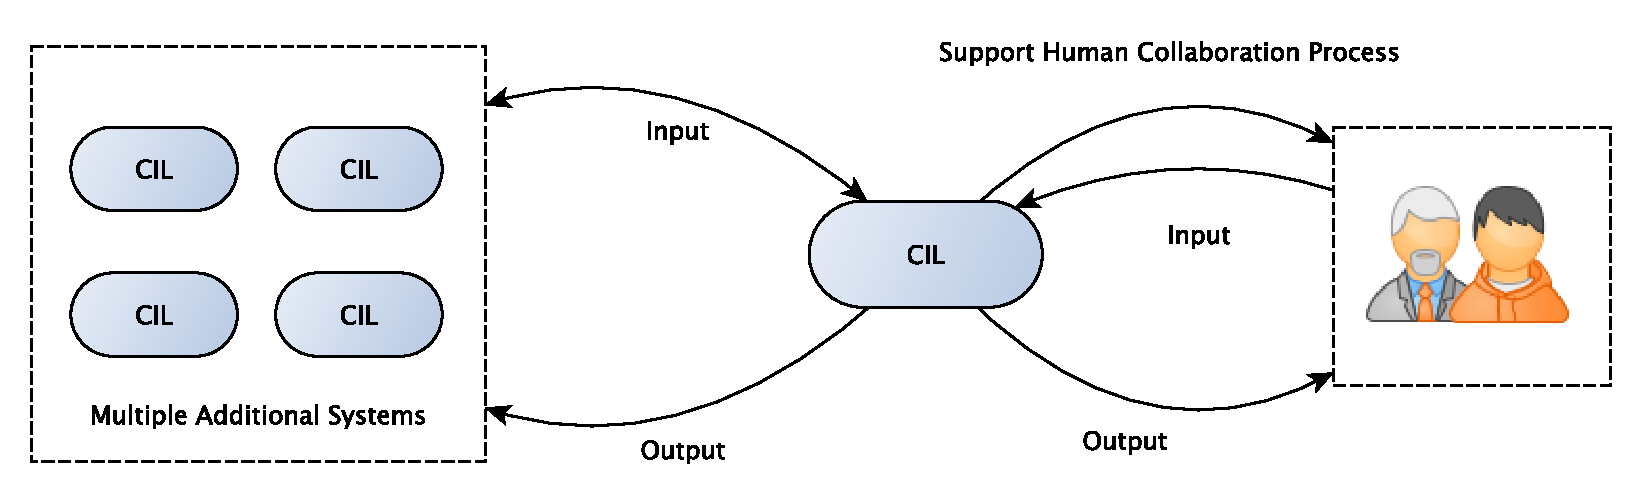
\includegraphics[width=3.5in]{images/CIL}
\caption{Interaction between heterogeneous systems in CIL.}
\label{fig:CIL}
\end{figure}
So the main difference to classical ML is the possibilty to adapt and optimise itself during run-time 
towards new situations without having been specifically trained for these use-cases, whereas classical ML 
systems have had to be fed with a sufficient amount of relevant training data\cite{CIL:sick}\cite{Organic:schloer}.
Furthermore, CIL systems interact with their environment in order to not rely on a single training data set. 
They collect data from several other sources (including humans) to validate already existing information and to 
gather additional data from other sources. In this way, CIL systems can be used in a lot of application areas where 
environments are constantly changing or training data is rarely available.
In general, we can still distinguish between \textit{dedicated} (concentrating mostly on one defined learning process, 
other interacting agents are largely human experts) and \textit{opportunistic} CIL (changing environments, heterogeneous 
sources of information)\cite{CIL:sick}, 
but we want to concentrate on general areas of application in this paper.

\section{Algorithmic Foundations}
\label{sec:algos}
Before we take a closer look at the applications and challenges of CIL, let's first consider the 
following existing machine learning strategies and algorithms. As already mentioned above, 
there is a multitude of definitions for the term ML\@. But primarily, Arthur Samuel 
coined this term in 1959. Of course, a lot has changed in this area since then, 
however, the definition that ML allows computers to solve problems without being 
specifically programmed to do so, is still valid today\cite{MLStudiesUsingCheckers:samuel}.

Over the last decades, ML has developed significantly and has become an area of
research interest for many different actors, which makes it difficult to divide learning 
strategies into several categories. Different researchers are using different approaches 
\cite{FoundationsOfML:mohri}\cite{Structure:corne}. 
However, in the following section I want to present five common strategies\cite{FoundationsOfML:mohri}.

\subsection{Supervised learning}
Basically supervised learning is the way of learning from labeled examples and making predictions 
for all unseen points. This is the most basic concept of ML and is used in a variety of applications 
where labeled data is easy to obtain. Spam mail detection for instance is a case where supervised learning 
techniques are - among others - used.
Many current mail programs have built-in spam detection which originally used
simple regular expressions in order to detect phrases commonly used in spam mails.
With state-of-the-art ML techniques it is not only possible for a mail program to 
query for a number of words but to recognise patterns of how spam mails are constructed and 
to adapt itself to new types of spam.
Supervised Learning methods have also been successfully applied in domains where it's 
important to extract information from images such as detecting and classifying 
objects or recognizing handwritten characters. Image 
recognition and OCR are therefore for example used in medical diagnosis to 
detect cancer on radiographs, in autonomous vehicles to detect obstacles and to 
stay on track or in post-offices to sort envelopes with hand-written addresses
\cite{DisciplineOfML:mitchell}. 


\subsection{Unsupervised learning}
In contrast to supervised learning, the learner receives only 
unlabeled training data and makes predictions for all unseen points in this concept. This technique is 
relatively similar to the way infants learn new things (e.g.\ learning a language) and 
is used, for example, in clustering data into groups, which we will discuss later\cite{BrainInf:holzinger}.
Furthermore, nearly all current search machines use unsupervised learning strategies in one fashion or another. 
They mainly use these techniques for \textit{(1) Ranking}, \textit{(2) User classification}\cite{DisciplineOfML:mitchell} 
in order to offer personalized search results and for \textit{(3) Query classification} in order to ``understand'' a 
users query and to provide further meaningful information. 

\subsection{Semi-supervised learning}
As the name suggests, the learner receives training data, which consists of both 
labeled as well as unlabeled data. Typically more unlabeled than labeled data.
This technique is mainly used in areas where data is easily accessible, 
but finding the right label is hard.
Most commercial applications for speech recognition are using this technique to train itself to 
recognise a user's speech input in order to perform further semantic analysis on
that data. Obtaining a sufficient amount of labeled data, for example the transcriptions of 
recorded audio files, would be expensive. Thus, unlabeled together with labeled data is being used 
to train a learner in a meaningful way.

\subsection{Reinforcement Learning}\label{reinforcement}
Reinforcement learning is probably the oldest approach and a potentially important one for CIL because 
it constantly tries to reinforce its learning process and improve its behavior. 
The learner constantly interacts with its environment to gain new information. A second instance interpretes the 
actions a learner carries out and rewards it depending on the actions outcome for the environment. The goal of 
the learner now is to maximize its reward over several repetitions. 
However, he is in conflict with using the information which has already been discovered by his actions 
or with getting more information through further actions. Reinforcement Learning has been successfully 
applied to various problems. 
Computer games usually offer a multiplayer mode where a user can interact and 
play the game even without a human opponent. For games with a small number of 
possible moves after each turn, and therefore a relatively small game tree containing 
all possible moves, the minimax algorithm\cite{Prog2:bachmaier} can be sufficient. 
It figures out which next move would minimize the worst-case scenario for all subsequent 
moves. Therefore, it needs to know all possible moves, which can easily become computationally 
infeasible for games like Chess or AlphaGo where a general move faces between 35 (Chess) and 
250 (AlphaGo) possible subsequent game states. 
Therefore, game artificial intelligences like AlphaGo are using Reinforcement Learning in order to gain 
experience by themselves\cite{Alpha:silver}.

%\subsection{Active Learning}\label{active}
%The goal of Active Learning is to interact with other agents in a clever way in order 
%to label already existing data points and thus achieve a similar performance with less available 
%information as in the method of supervised learning. To achieve this, 
%the learner needs a selection strategy\cite{ActiveToDedicated:calma} that decides whether 
%an action has enough information content to label a data point or not.
%\notes{[Example needed.]}


\section{When using CIL is helpful}\label{AdvantageOfCIL}
In established ML systems, a separate model must be developed and trained in advance for 
each specific application. ML systems therefore have a relatively narrow application frame. 
The idea behind CIL systems is that they learn, self-organize and improve knowledge throughout their lives. 
They collect information from various sources and evaluate the obtained data, so that they 
can solve problems together with other technical and human agents in a 
collaborative and interchangeable way\cite{CIL:sick}.
The CIL approach therefore deliberately integrates other intelligent systems 
(people and machines) into the decision-making process in order to ensure that the individual entities 
can solve otherwise difficult problems much easier.
Another difference to classical approaches is the mutual benefit. 
Machines not only benefit from training data of other agents, but also provide 
an own contribution to actively support human collaboration processes by 
recognising their wishes and needs and reacting accordingly\cite{CIL:sick}.

\section{Classification of CIL in Organic Computing}
The term ``organic'' can be intuitively described as structures being live-like and making decisions on their own. 
A more formal way of characterizing even technical systems as organic is checking the applicability of 
so-called self-x-properties\cite{Organic:schloer}\cite{Organic:schmeck}.

\subsection{Self-Configuration}
A system is being called self-configurable, if it can modify its parameters on its own.
CIL systems configure themselves in the sense that they are not aligned by developers to any narrow application 
case but adapt their behavior in the current environment to its desired purpose.

\subsection{Self-Optimization}
In order to deliver reasonable output, a systems needs to constantly improve itself over its lifetime. Thus, parts of 
the system have to analyze decisions made during run-time.
CIL systems optimize themselves by applying various strategies of ML to expand their knowledge.

\subsection{Self- Healing and Protection}
Furthermore, if systems work in changing environments and interact with other agents, they're always exposed to 
the risk of failure. Therefore, organic systems need to detect failures (either triggered by an own action or by an intruder) 
and fix the faulty part.
CIL systems in particular need to implement these features due to their desired interaction with multiple 
other heterogeneous systems.

\subsection{Self-Explanation}
Ultimately, CIL systems need to stay self-explanatory. Due to the fact that they interact with a lot of other systems, over 
different communication channels and in changing environments, networks of a massive amount of intelligent systems will arise. 
Comprehending and understanding these structures even after a long period of time will be a difficult but important research 
area in the field of CIL systems\cite{Organic:schloer}.

\section{Application examples}
In the following section we will discuss some interesting application examples.

\subsection{Clustering}
Clustering is the perfect example of a starting point without sufficient information about an amount of data. 
The basic goal here is to divide a data set into homogeneous groups of individual data points in order to create structure in it.
In this context data points must be checked for similarity in some way.
Clustering is used, for example, in most recommendation systems of popular internet applications 
(\textit{Netflix} movie recommendations, \textit{YouTube} Video Tags\cite{YouTube:pasca}) to group similar tags or find groups 
of people with a similar taste in movies.
Furthermore, clustering can be used to identify communities in social networks, for example for target-advertising, or to cluster location-data so that "important places" of a person can be identified\cite{DJ:frankowski}.

Unfortunately, real-world data in these areas is often unclean, contains false or unwanted data and is often present in 
dimensions $>$3, so that people alone, who are otherwise very good at recognizing similarities in dimensions $\le3$, are dependent on ML and vice-versa.

There are different approaches to cluster data into homogeneous groups. One of them is the k-Means algorithm\cite{FoundationsOfML:mohri}. In the beginning it requires the number of $k$ clusters it is supposed to find. It then proceeds as follows: 
\begin{enumerate}
    \item Randomly place $k$ centroids in space (these represent the center of a single cluster).
    \item Assign each item in space to its nearest centroid.
    \item Move each centroid to the center of all items assigned to it.
    \item Repeat (2) and (3) until the assignments of the items no longer change.
\end{enumerate}
%It then randomly places $k$ centroids in space, which should represent the center of a cluster, and assigns each item to the nearest centroid. After the assignment, each centroid is placed at the center of all items assigned to it. This process of assigning the items and moving the centroids to
%the center is now repeated until the assignments of the items no longer change.

What all cluster algorithms have in common is that they need a way to compare data points for similarity respectively distance 
in order to find centers.
Classically, data points are tried to be displayed in an n-dimensional metric space and, for example, their Euclidean distance is measured for similarity.
The Euclidean distance between two data points $p = (p_1, p_2, \dots, p_n)$ and $q = (q_1, q_2, \dots, q_n)$ and thus their
similarity, when a small result means more similar, is defined as
\begin{equation*}
    similarity(p, q) = \sqrt{\sum_{i=1}^{n} (q_i - p_i)^{2}}.
\end{equation*}

Since data is usually multidimensional, i.e.\ much larger than three, suitable attributes must be selected for the comparison. 
However, the problem here is that similarity functions are influenced by subjective factors, since experts from different 
fields also find different partial aspects of the amount of data that is examined interesting.
Therefore, the CIL approach can provide a decisive advantage in this case, as the knowledge and assessment of 
different experts and other systems can be used to make such decisions.
An interesting interactive approach follows\cite{DJ:frankowski}, which creates a personal gazetteer from a user's location data 
by interactively asking the right questions after cleaning the data from unwanted noise.

\subsection{Health Domain}
Also and especially in medical diagnosis, doctors are often confronted with a very small amount of data.
For rare diseases in particular, there are not enough training examples to use classical ML approaches efficiently and with a low error rate in practice.
In many areas, such as emergency surgery, results are often required within a very short time, which makes pure ML techniques useless in a lot of cases.
After successfully completing their medical studies, however, doctors, even with relatively little experience, already have the ability to examine and classify X-rays sufficiently accurately for various diseases and anomalies.
In these cases the intuitiveness of one or more people can profitably support the CIL system.

Another area of application in the field of medical research also takes advantage of human puzzle-solving intuition. 
For years the project "foldit" of the University of Washington has achieved remarkable results\cite{Foldit:results} from the gamification of a problem related to biology.
The researchers have developed a game that helps them to optimize and predict possible protein structures with the help of 
players\cite{Foldit:web}.
Proteins can fold in a number of different ways. Even with smaller proteins, the number of possible folds can be extremely high due to their many degrees of freedom.
The aim of the game is to determine the optimal folding and thus the "most comfortable" state of a protein in order to be able to develop appropriate drugs for and with this shape.
Since the structure determines the function of a protein\cite{Foldit:web}, new forms can also be used to treat diseases such as AIDS or cancer more effectively.

So we already see a system in this field that at least involves the human being as a collective form of knowledge acquisition in the solution of complex problems, even if not directly with technical systems.
The next step towards CIL in this area could be to incorporate the results of human puzzle-solving into the calculations and decisions of ML systems in order to proactively support humans (bi-directional way of inputs, see Section~\ref{sec:intro}) in finding solutions 
for example by excluding unpromisingfls.


\subsection{Industry and Manufacturing}
The primary goal in manufacturing is to keep production up and running under almost all circumstances. 
Even short downtimes of production lines result in high sales losses for companies.
This is why it is important to keep an eye on the wear of work equipment, production lines and the condition of machines in general at all times.
Current systems already use various ML techniques\cite{Manu:wuest} to cover these applications.

For CIL-systems, it is conceivable, in addition to the sensor data used by the devices to "measure" wear, to call in expert knowledge, so that rare cases that are easily recognisable as a suspicious situation for humans, can be identified at an early stage by the whole system.
In this process, a CIL system must estimate at runtime which expert should be asked what and when in order 
to achieve maximum information content.

\section{Challenges and future directions}
Since the area of Collaborative Interactive Learning is a very new field of research, there is still a lot of 
research to be done in the areas of continuous knowledge acquisition 
and evaluation from several heterogeneous sources (Internet, expert knowledge, etc.), 
as well as the interaction with multiple other agents (humans and other CIL systems), 
especially when systems have to adapt to changing situations during their lifetime.

Not only technical difficulties have to be overcome, but also social ones. In order to use ML techniques effectively, 
at least a minimum amount of data has to be provided in order to be analyzed. To do this, we need to decide 
to what extent we are willing to disclose our data for the benefits of CIL systems and ML in general.
Inhibitions in human-machine communication and interaction must also be overcome for CIL systems to be used 
successfully and productively.

\begin{thebibliography}{1}
\bibitem{ML:mitchell}
    Mitchell, T. M. (1997). Machine learning. 1997. Burr Ridge, IL: McGraw Hill, 45(37), 870-877.
\bibitem{FoundationsOfML:mohri}
    Mohri, M., Rostamizadeh, A., \& Talwalkar, A. (2012). Foundations of machine learning. MIT press.
\bibitem{DisciplineOfML:mitchell}
    Mitchell, T. M. (2006). The discipline of machine learning (Vol. 9). Carnegie Mellon University, School of Computer Science, Machine Learning Department.
\bibitem{Prog2:bachmaier}
    Bachmaier, C. (2017). Lecture. Programming II\@. Faculty for Informatics and Mathematics, University of Passau, Germany.
\bibitem{CIL:sick}
    Sick, B., Oeste-Rei{\ss}, S., Schmidt, A., Tomforde, S., \& Zweig, A. K. (2018). Collaborative Interactive Learning. Informatik-Spektrum, 41(1), 52-55.
\bibitem{Structure:corne}
    Corne, D., Dhaenens, C., \& Jourdan, L. (2012). Synergies between operations research and data mining: The emerging use of multi-objective approaches. European Journal of Operational Research, 221(3), 469-479.
\bibitem{ActiveToDedicated:calma}
    Calma, A., Leimeister, J. M., Lukowicz, P., Oeste-Rei{\ss}, S., Reitmaier, T., Schmidt, A., \dots \& Zweig, K. A. (2016, April). From active learning to dedicated collaborative interactive learning. In ARCS 2016; 29th International Conference on Architecture of Computing Systems; Proceedings of (pp. 1-8). VDE.
\bibitem{BrainInf:holzinger}
    Holzinger, A. (2016). Interactive machine learning for health informatics: when do we need the human-in-the-loop?. Brain Informatics, 3(2), 119-131.
\bibitem{Alpha:silver}
    Silver, D., Hassabis, D. (2016, January). AlphaGo: Mastering the ancient game of Go with Machine Learning. Google AI Blog. Retrieved from \url{https://ai.googleblog.com/2016/01/alphago-mastering-ancient-game-of-go.html} on August 24, 2018. 
\bibitem{MLStudiesUsingCheckers:samuel}
    Samuel, A. L. (1959). Some studies in machine learning using the game of checkers. IBM Journal of research and development, 3(3), 210-229.
\bibitem{Organic:schloer}
    M{\"u}ller-Schloer, C., von der Malsburg, C., \& W{\"u}rt, R. P. (2004). Organic computing. Informatik-Spektrum, 27(4), 332-336.
\bibitem{Organic:schmeck}
    Schmeck, H. (2005, May). Organic computing-a new vision for distributed embedded systems. In Object-Oriented Real-Time Distributed Computing, 2005. ISORC 2005. Eighth IEEE International Symposium on (pp. 201-203). IEEE.
\bibitem{DJ:frankowski}
    Zhou, C., Frankowski, D., Ludford, P., Shekhar, S., \& Terveen, L. (2004, November). Discovering personal gazetteers: an interactive clustering approach. In Proceedings of the 12th annual ACM international workshop on Geographic information systems (pp. 266-273). ACM.
\bibitem{YouTube:pasca}
    Toderici, G., Aradhye, H., Pasca, M., Sbaiz, L., \& Yagnik, J. (2010, June). Finding meaning on youtube: Tag recommendation and category discovery. In Computer Vision and Pattern Recognition (CVPR), 2010 IEEE Conference on (pp. 3447-3454). IEEE.
\bibitem{Foldit:web}
    The Science Behind Foldit. (n.d.). University of Washington, Departments of Computer Science \& Engineering and Biochemistry. Retrieved from \url{https://fold.it/portal/info/about} on June 29, 2018. 
\bibitem{Foldit:results}
    Boyle, A. (2011, September). Gamers solve molecular puzzle that baffled scientists. Cosmic Log.\\
    Retrieved from \url{https://cosmiclog.nbcnews.com/_news/2011/09/18/7802623-gamers-solve-molecular-puzzle-that-baffled-scientists} on June 29, 2018.
\bibitem{Manu:wuest}
    Wuest, T., Weimer, D., Irgens, C., \& Thoben, K. D. (2016). Machine learning in manufacturing: advantages, challenges, and applications. Production \& Manufacturing Research, 4(1), 23-45.
\end{thebibliography}


\end{document}


